\documentclass[a4paper,12pt]{article}
\usepackage[italian]{babel}
\usepackage[utf8]{inputenc}
\usepackage[T1]{fontenc}
\usepackage{geometry}
\usepackage{fancyhdr}
\usepackage{fancyvrb}
\usepackage{graphicx}
\usepackage{titlesec}
\usepackage{pifont}
\usepackage{verbatim}
\usepackage{caption}
\usepackage{indentfirst}
\usepackage{amsmath}
\usepackage{datetime}

% Page setup
\geometry{margin=0.8in}
\pagestyle{fancy}
\fancyhf{}
\rhead{\thepage}
\renewcommand{\headrulewidth}{0pt}

\title{\textbf{GaetanoBros}}
\author{Alessandro Amella, Michele Garavani, Simone Ballo}
\date{\formatdate{2}{9}{2023}}

\begin{document}
\maketitle

\section{Introduzione e architettura del software}
Abbiamo voluto sviluppare la nostra versione del gioco, denominata \textbf{GaetanoBros}, con l'obiettivo di creare un codice altamente modulare e ben strutturato. Alcuni principi che ci siamo prefissati sono:
\begin{itemize}
\item \textbf{Principio di Singola Responsabilità}: a ogni classe corrisponde una e una sola responsabilità (una classe per il rendering, una per i nemici, una per il timer, ecc.).
\item \textbf{Gerarchia di Classi}: sfruttare l'ereditarietà ove possibile.
\item \textbf{Separation of concerns}: separare chiaramente le responsabilità di ciascuna entità tramite le proprie classi o file header dedicati.
\item \textbf{Encapsulation}: nascondere i dettagli di implementazione delle classi mantenendoli privati, fornendo esclusivamente interfacce pubbliche per interagire con il resto del codice.
\end{itemize}

Questo approccio ci ha permesso di ottenere un codice altamente modulare, il quale ha permesso di apportare facilmente modifiche, anche drastiche. Inoltre ha semplificato l'interazione tra i vari componenti del gruppo, poiché hanno potuto utilizzare le interfacce pubbliche delle classi senza dover conoscere i dettagli di implementazione sottostanti.


\section{Implementazione}
\subsection{Codice condiviso e costanti di gioco}
Per rendere il codice del nostro gioco più modulare e manutenibile, evitando di fare un \textit{hard-coding} di valori specifici all'interno del codice, abbiamo separato le costanti e le funzioni condivise in file distinti nella cartella \texttt{src/shared}. Il file \texttt{settings.hpp} contiene svariate costanti e strutture dati che regolano i vari comportamenti del gioco, come le dimensioni della finestra di gioco, mentre il file \texttt{functions.hpp} contiene funzioni comuni usate ampiamente in diverse parti del codice, come la funzione \texttt{clamp()} o \texttt{collides()}.

\subsection{Gestione centralizzata}
Abbiamo subito pensato che, per unire tutti gli aspetti del gioco, avremmo avuto bisogno di una classe centralizzata che si occupasse di gestire il flusso complessivo del gioco, l’unica classe a conoscenza di tutte le altre classi. Abbiamo chiamato tale classe \texttt{GameManager}. Tale classe, infatti, gestisce l'inizializzazione del gioco, il ciclo di gioco principale, le interazioni dei giocatori, le collisioni, il rendering, le condizioni di game over, e in generale ogni situazione in cui viene richiesta la conoscenza di dati tra classi isolate tra loro (ad esempio, le collisioni tra il player e i nemici). Tutte le altre classi, direttamente o indirettamente, vengono implementate in \texttt{GameManager}.

\subsection{Logica di tick}
Il nostro gioco usa una \textbf{logica di tick} per aggiornare lo stato del gioco e gestire gli eventi in modo sincronizzato. Un tick è un'unità di tempo che rappresenta un intervallo fisso, definito dalla costante \texttt{TICK\_INTERVAL} nel file \texttt{src/shared/settings.hpp}. Ad ogni tick, il gioco esegue una serie di operazioni che influenzano il comportamento degli oggetti e delle entità nel gioco.

Per implementare la logica di tick, abbiamo definito la classe \texttt{GameTimer}, che è una classe che misura il tempo trascorso a partire da un certo istante di tempo. Un oggetto \texttt{GameTimer} è naturalmente istanziato all'interno di \texttt{GameManager}, il quale ha anche una lista di puntatori alle classi che devono essere aggiornate ad ogni tick, come la classe \texttt{Player}, \texttt{Enemy}, \texttt{Projectile}, ecc.

\texttt{GameManager} esegue un loop infinito in cui controlla se è il momento di fare un tick, chiamando il metodo \texttt{should\_tick()} di \texttt{GameTimer}. Questo metodo restituisce \texttt{true} se il tempo trascorso dall'ultimo tick è maggiore o uguale a \texttt{TICK\_INTERVAL}: in tal caso, \texttt{GameManager} chiama a sua volta il metodo \texttt{tick()} su tutte le classi di cui è a conoscenza sul quale tale metodo è definito, le quali chiameranno, a loro volta, il medesimo metodo sulle classi di cui esse sono a conoscenza. In questo modo, la logica di tick si propaga da una classe all'altra, creando una catena di chiamate che coinvolge tutte le classi che devono essere aggiornate col procedere del tempo.

\subsection{Rendering del gioco}

Per visualizzare il gioco sullo schermo tramite la libreria \textit{ncurses} abbiamo creato una classe \texttt{GameRenderer} che disegna gli elementi del gioco, come il giocatore, i nemici, i powerup, ecc. Essa è l'unica classe a conoscenza di \textit{ncurses}: nell'obiettivo di scrivere codice modulare, si rende possibile cambiare la libreria di rendering solamente apportando opportune modifiche alla classe \texttt{GameRenderer}. Quest'ultima possiede alcuni attributi che sono puntatori alle classi che contengono lo stato del gioco, e alcuni metodi che usano le funzioni di \textit{ncurses} per disegnare le componenti del gioco. Il metodo principale è \texttt{render\_game()}, che aggiorna la visualizzazione del gioco (viene chiamato ad ogni tick da \texttt{GameManager}). \\

È importante specificare che, su \textit{ncurses}, l'asse $y$ è invertita ($y = 0$ rappresenta la parte superiore dello schermo). Nell'intera logica di gioco si usa, invece, una base di coordinate standard pari al piano cartesiano, con la retta $y = 0$ indicante la parte inferiore dello schermo. \texttt{GameRenderer} possiede quindi dei metodi interni, come \texttt{translate\_position()}, per traslare le posizioni ai valori adatti per \textit{ncurses}.

\subsection{List}
Per avere una struttura dati dinamica che ci permette di rappresentare una sequenza di oggetti, abbiamo creato la classe \texttt{List}, decidendo di implementarla come lista concatenata semplice, sfruttando la \textbf{programmazione generica} offerta da C++: la classe viene definita come \textit{classe template}, permettendoci di utilizzarla estensivamente nel codice con qualunque tipo di dato (\texttt{int}, \texttt{char}, \texttt{Platform}, \texttt{Room*}, …).
Abbiamo naturalmente definito ed esposto metodi pubblici per l'accesso e la modifica ai dati (\texttt{push}, \texttt{pop}, \texttt{at}, \texttt{length}, \texttt{contains}, \texttt{clear}, …).

\subsection{Gestione input}
Abbiamo deciso di raggruppare la gestione degli input da tastiera dell'utente nella classe \texttt{InputManager}. Ciò che succede se i tasti vengono premuti viene definito nelle classi specifiche. Ad esempio, le azioni dei comandi del giocatore sono definite nella classe \texttt{Player}. I comandi dello shop sono gestiti nella classe \texttt{Shop}. Il tasto '\texttt{q}', che permette di uscire dal gioco, viene gestito nella classe \texttt{GameManager}. 

\subsection{Entità}
Per implementare le varie entità del progetto abbiamo pensato di usufruire dell’ereditarietà tra classi. Abbiamo iniziato con la classe base \texttt{StaticEntity}, usata come classe astratta per rappresentare una generica entità la cui posizione resta costante nel tempo, alla base di molte altre classi.
\begin{figure}
\centering
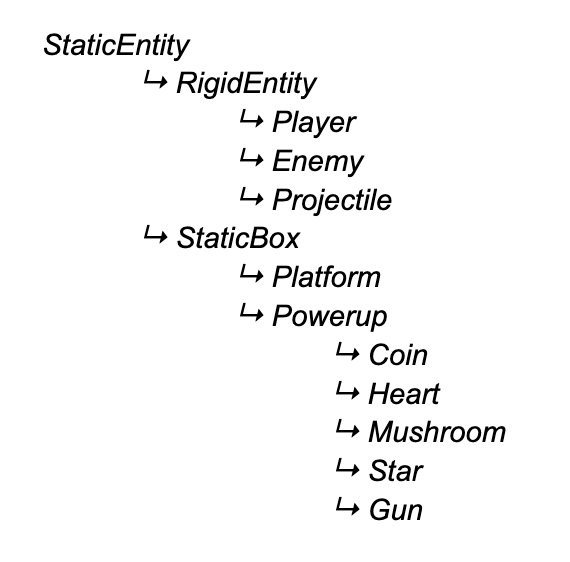
\includegraphics[width=0.4\textwidth]{hierarchy.png}
\captionsetup{labelformat=empty}
\caption{\small Uno schema con la gerarchia di classi partendo da \texttt{StaticEntity}.}
\end{figure}
%\begin{comment}
%In seguito uno schema con la gerarchia di classi partendo da \texttt{StaticEntity}.
%\begin{Verbatim} [commandchars=\\\{\}]
%StaticEntity
%	\ding{212} RigidEntity
%		\ding{212} Player
%		\ding{212} Enemy
%		\ding{212} Projectile
%	\ding{212} StaticBox
%		\ding{212} Platform
%		\ding{212} Powerup
%			\ding{212} Coin
%			\ding{212} Heart
%			\ding{212} Mushroom
%			\ding{212} Star
%			\ding{212} Gun
%\end{Verbatim}
%\end{comment}


Per creare i potenziamenti e la valuta, in quanto entità, abbiamo usufruito dell’ereditarietà. Abbiamo prima di tutto creato la classe \texttt{StaticBox}, composta di due punti, che possono formare un rettangolo rappresentato dalle coordinate in basso a destra e in alto a sinistra.
Abbiamo poi creato la sottoclasse \texttt{Powerup}, da cui vengono create le classi con i vari potenziamenti singoli. Le abilità dei potenziamenti vengono come al solito gestite da \texttt{GameManager} (ad esempio, essendo in carico delle collisioni, farà sì che il player non subisca danno quando esso possiede il powerup \textit{stella} e viene colpito da un nemico).\\

Per implementare le "\textit{rigid entities}", ovvero le entità dotate di velocità, abbiamo aggiunto attributi importanti come ad esempio:
\begin{itemize}
\item Le velocità orizzontali e verticali dell’entità.
\item Un riferimento alle regioni di inizio e di fine, alle piattaforme, all’altezza del pavimento e del soffitto della stanza attuale.
\item Un metodo \texttt{tick()} che controlla le collisioni, aggiorna la velocità e la posizione.
\end{itemize}

Da questa classe, chiamata \texttt{RigidEntity}, derivano altre classi chiave nel gioco come \texttt{Player}, il quale possiede altri aspetti importanti come le capacità di salto, i tasti per muoversi, e le interazioni con i powerups (tra cui la gestione di monete e salute).

Similmente vengono create anche le classi figlie di \texttt{RigidEntity} che gestiscono nemici e proiettili.

\subsection{Livelli}
Un altro aspetto molto importante del gioco è la suddivisione in livelli. Abbiamo pensato di implementare una struttura a stanze (classe \texttt{Room}). Il player può andare avanti e indietro tra le stanze entrando nelle \textbf{regioni di inizio e fine} (implementate come \texttt{StaticBox}). Una stanza è definita con vari parametri, tra cui una lista delle sue piattaforme, le sue dimensioni, l’altezza del pavimento e del soffitto, regioni di inizio e fine: questi parametri sono ciò che rendono le stanze diverse tra loro.
I layout delle varie stanze, ciascuno definito all'interno di un file \texttt{layout<i>.cpp}, sono tutti accessibili attraverso i metodi pubblici di \texttt{Maps}, creata per combinare i layout in un'unica classe.

La classe \texttt{LevelManager}, la quale contiene una lista di stanze istanziabili (che punta alle mappe salvate all'interno di \texttt{Maps}), si occupa di gestire il cambiamento di stanza. Essa possiede: 
\begin{itemize}
\item \texttt{List<RoomState> visited\_rooms}: una lista di oggetti \texttt{RoomState}, i quali associano un puntatore di una determinata stanza (\texttt{Room*}) alla difficoltà alla quale si sta giocando tale stanza (\texttt{int}).
\item \texttt{int cur\_visited\_room\_index}: un indice che rappresenta il \texttt{RoomState}, all'interno della lista \texttt{visited\_rooms}, al quale si trova attualmente il player.
\item \texttt{get\_cur\_room()}: un metodo pubblico che restituisce un puntatore alla stanza attuale, pari alla stanza dell'elemento \texttt{visited\_rooms} all'indice \texttt{cur\_visited\_room\_index}.
\end{itemize} 

In tal modo il player può fare avanti e indietro tra le stanze e la difficoltà viene impostata correttamente.
Quando il giocatore si posiziona alla regione di inizio di una stanza (ed essa non è la prima stanza), allora l’indice \texttt{cur\_visited\_room\_index} viene decrementato e di conseguenza \texttt{get\_cur\_room()} restituirà la stanza precedente.
In modo analogo, se il player si trova alla regione di fine, allora l'indice viene incrementato. 

Se l’indice è già a \texttt{visited\_rooms.length() - 1}, allora \texttt{LevelManager} provvede a istanziare una nuova stanza scelta casualmente, inserendola all'interno di \texttt{visited\_rooms} con tanto di nuova difficoltà, pari alla $\text{difficoltà precedente} + 1$.

Prima di incrementare l'indice, \texttt{LevelManager} chiama un apposito metodo per istanziare i nemici casualmente, di numero pari alla difficoltà, e powerup e monete, tentando di inserire casualmente almeno $2$ monete e un numero di powerup pari a $y = \max\left(-\sqrt{x} + 4, 1\right)$. \\

Quando il player muore e riavvia il gioco, l’indice viene riportato a 0 e gli elementi della lista di stanze visitate svuotata, ma la difficoltà, come da consegna, viene mantenuta.

\subsection{Shop}

Abbiamo infine creato la pagina dello shop, con la sua interfaccia grafica e le sue funzionalità (comprare potenziamenti). Abbiamo poi aggiunto l’istanza dello shop in \texttt{GameManager}, facendo in modo che lo shop compaia all’inizio del gioco e \textbf{ogni tre stanze}.

\appendix
\section{Contatti}

\centering

Alessandro Amella - alessandro.amella@studio.unibo.it - 0001070569

Michele Garavani - michele.garavani@studio.unibo.it - 0001079937

Simone Ballo - simone.ballo@studio.unibo.it - 0001069408

\end{document}
